%\chapter{Result and Discussion}
\section{Result}
As presentation about our result, in this section we introduce about MAELab software, the parameters used in execution and the discussion about the result.
\subsection{New interface}
The results of this internship are integrated into IPM\footnote{Image Processing for Morphometrics} software, but the software interface was reorganized (figure \ref{fig:44}). Besides the functions of previous version, the clients can be use new functions to segment image or automatic extraction landmarks from image.
\begin{figure}[h!]
\centering
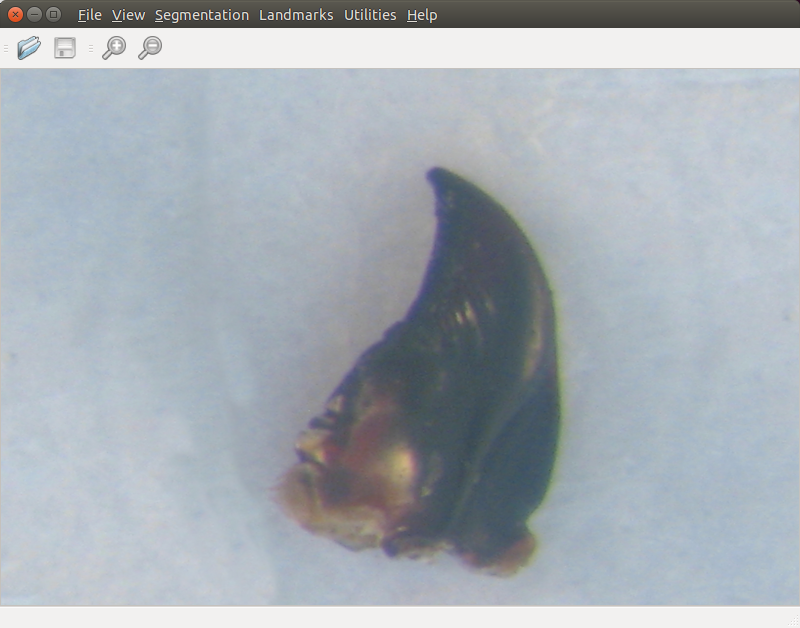
\includegraphics[width=0.7\textwidth]{./images/software}
\caption{The graphic user interface of MAELab software}
\label{fig:44}
\end{figure}~\\
The software provides adequately functions to process on biological image. Specially, the menu \textbf{Landmarks} contains the main result of this internship. It provides clients the functions automatically estimation landmarks and analysis the result from estimated landmarks. The process can be finished on an image or a list of images.
\begin{figure}[h!]
\centering
\subfloat[MAELab software]
{\label{fig:451}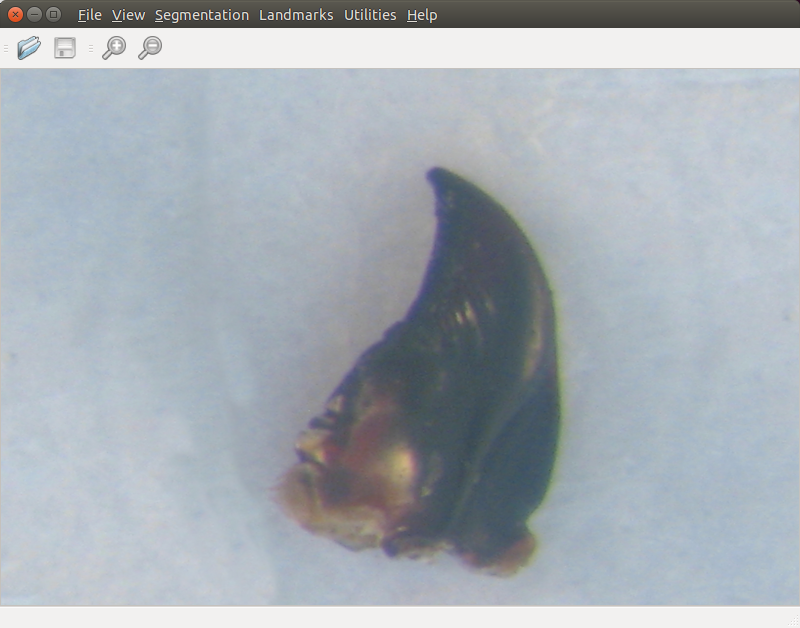
\includegraphics[width=0.45\textwidth]{./images/software}}~~
\subfloat[MAELab with Segmentation menu]
{\label{fig:452}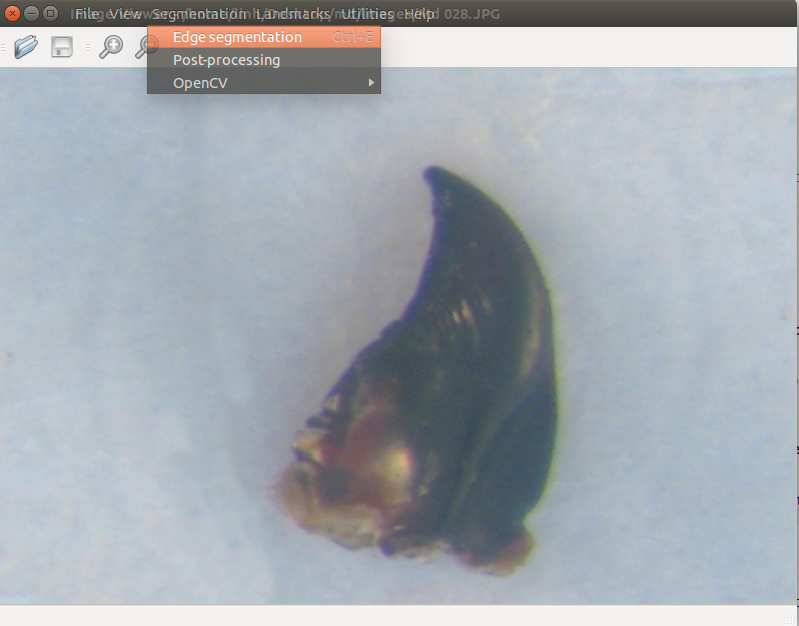
\includegraphics[width=0.45\textwidth]{./images/newiface1}}\\
\subfloat[MAELab with Landmarks menu]{\label{fig:453}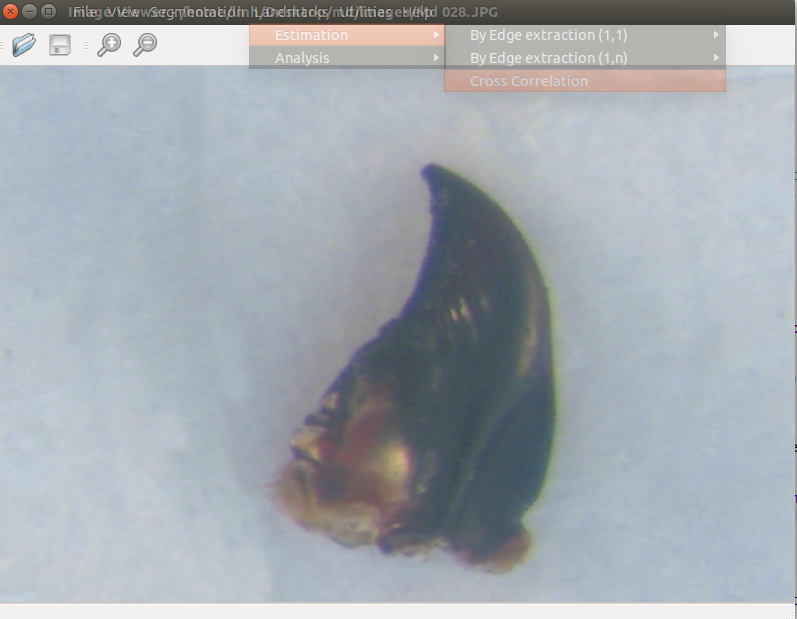
\includegraphics[width=0.45\textwidth]{./images/newiface2}}~~
\subfloat[MAELab with Utilities menu]
{\label{fig:454}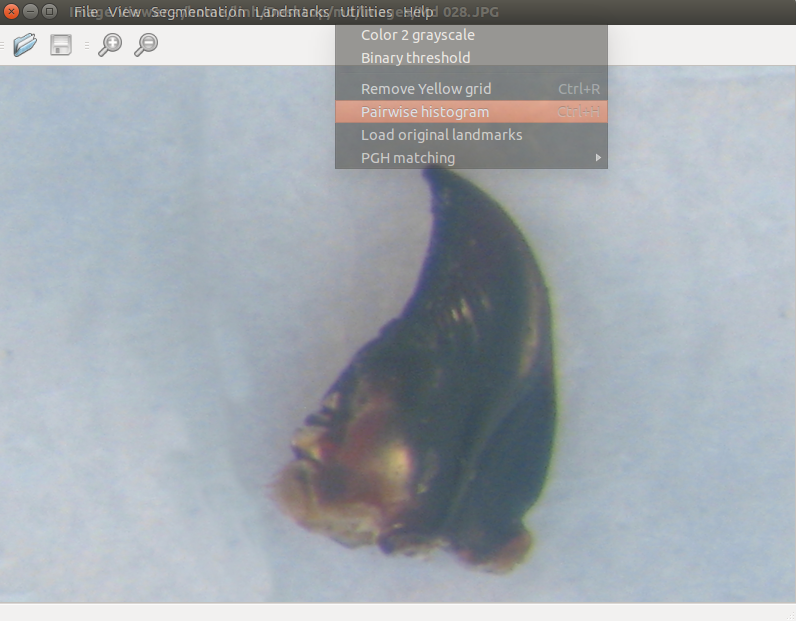
\includegraphics[width=0.45\textwidth]{./images/newiface3}}
\caption{The MAELab software with its menu}
\label{fig:45}
\end{figure}~\\[0.2cm]
Besides, the other functions developed in MAELab software are:
\begin{itemize}
\item Image segmentation by analysing histogram (in \textbf{Segmentation} menu)
\item Removing the yellow grid on image (in \textbf{Utilities} menu)
\item Loading the manual landmarks (in \textbf{Utilities} menu)
\item Computing the pairwise geometric histogram (PGH) of image (in \textbf{Utilities} menu)
\item Computing the measure metric between PGHs by Bhattacharya, Chi-Squared or Intersection method (in \textbf{Utilities} menu)
\end{itemize}
\subsection{Experimentation}
The experimentation is deployed on two machines with difference equipment:
\begin{itemize}
\item Machine 1: Intel(R) Core(TM) 2 Duo CPU T8100 2.1GHz, 2 GB of RAM
\item Machine 2: Intel(R) Core(TM) i7-4790 CPU 3.6GHz, 16 GB of RAM
\end{itemize}
The testing data is two set of biological images: \textit{Right mandible and left mandible}. Each dataset includes 293 images(3264 x 2448). However, the data was filtered by suppressing the bad images in the both datasets. The bad images includes the empty images and broken images (images contain the broken object). They are showed as below:
\begin{multicols}{3}
\begin{itemize}
\item Md 004.JPG
\item Md 146.JPG
\item Md 238.JPG
\item Mg 003.JPG
\item Mg 007.JPG
\item Mg 040.JPG
\item Mg 066.JPG
\item Mg 159.JPG
\item Mg 248.JPG
\item Mg 292.JPG
\end{itemize} 
\end{multicols}
Because the estimation method has several steps, we decide focus on some steps of method, such as segmentation and estimation. For each step, we compute the execution time on one image and a list of images. Then we compare the runtime between two examination systems (see in table \ref{table_runtime1} and table \ref{table_runtime2}).

Machine 1:
\begin{table}[h]
	\centering
	\begin{tabular}{|c|c|c|}
		\hline
		No of images & Segmentation(second) & Estimation(second) \\ \hline
		1 & 0.844 & 31.4245   \\ \hline
		290 & 571.576 & 13000.9131   \\ \hline
	\end{tabular}	
	\caption{The runtime of program on machine 1}		
	\label{table_runtime1}
\end{table}

Machine 2:
\begin{table}[h]
	\centering
	\begin{tabular}{|c|c|c|}
		\hline
		No of images & Segmentation(second) & Estimation(second) \\ \hline
		1 & 0.27782 & 10.4392   \\ \hline
		286 & 171.589 & 4665.79   \\ \hline
	\end{tabular}
	\caption{The runtime of program on machine 2}
	\label{table_runtime2}
\end{table}
Based on the runtime tables, the most of runtime stays in stage of estimation. This is the time to execute two steps: estimated landmarks (by PHT) and refine landmarks (by template matching). Hence, it also depend on the configuration of system.
\subsection{Parameters}
In our program, we use these parameters for the methods:
\begin{itemize}
\item The best segmentation obtained from choosing a good threshold value. In the program, Canny algorithm is applied to segment the image. Thus, the ratio between \textit{lower threshold : upper threshold} is important to get a good result. And the ratio is: \textit{1 : 3} (in class \texttt{Image}, method \texttt{getEdges}), this ratio has been chosen experimentally. The lower value is 1 * \textit{threshold} value and the upper value is 3 * \textit{threshold} value. The \textit{threshold} value is identified by analysing the histogram of image. 
\item The angle and distance accuracy used in constructing the PGH matrix and calculate the measure distance between PGHs. The angle accuracy can be 90 (0.5 * 180), 180, 360 (2 * 180), 720(4 * 180), 1080(6 * 180), 2160(12 * 180) degree. The distance accuracy can be 250, 500 or 1000 columns. The \textbf{default value} in program is \textbf{180} degree for angle accuracy, and \textbf{250} for the distance accuracy. 
\item During applying the Probabilistic Hough Transform, to reduce the time complexity during training, we consider the pair of closet lines. And the parameters used to indicate the closet line are (used in method \texttt{closetLine}, class \texttt{PHoughTransform} ):
	\begin{itemize}
		\item Length of each line greater than \textbf{60} pixels
		\item Angle between two lines greater than \textbf{15} degree
		\item Perpendicular distance from one of two endpoints of a line to other line less than \textbf{5} pixel.
	\end{itemize}
The conditions to predicate two pairs of lines are similar (used in method \texttt{similarPairLines}, class \texttt{PHoughTransform}):
	\begin{itemize}
		\item Subtraction between angle of two pair of lines is less than \textbf{1}
		\item Subtraction between ratio couple of scene lines and reference lines is less than \textbf{1}
		\item Subtraction between distance of two pair of lines is less than \textbf{2}
	\end{itemize}
\item The size of bounding box around the reference landmarks used for estimating landmarks by cross-correlation method or computes the estimated centroid is \textit{400} pixels (used in method \texttt{crossCorrelation and crossCorrelationDistance}, class \texttt{ImageViewer})
\item The size of bounding box around reference landmarks and estimated landmarks used to refine the estimated landmarks or compute the estimated centroid are \textit{400} pixels and \textbf{1400} pixels, respective.(used in method \texttt{getLandmarks and tplMatchingDistance}, class \texttt{ImageViewer})
To increase the flexible of program, all parameters was placed in the resources files (\textbf{data/resources} folder). For each group of parameters, the parameters are put in a file.
\end{itemize}
\subsection{Results}
The automated landmark identification is examined on two data sets: \textit{right mandible and left mandible}. And the landmarks are extracted: 18 landmarks for each \textit{right mandible} image, 16 landmarks for each \textit{left mandible} image.\\
\begin{figure}[h!]
\centering
\subfloat[The scene image]{\label{fig:461}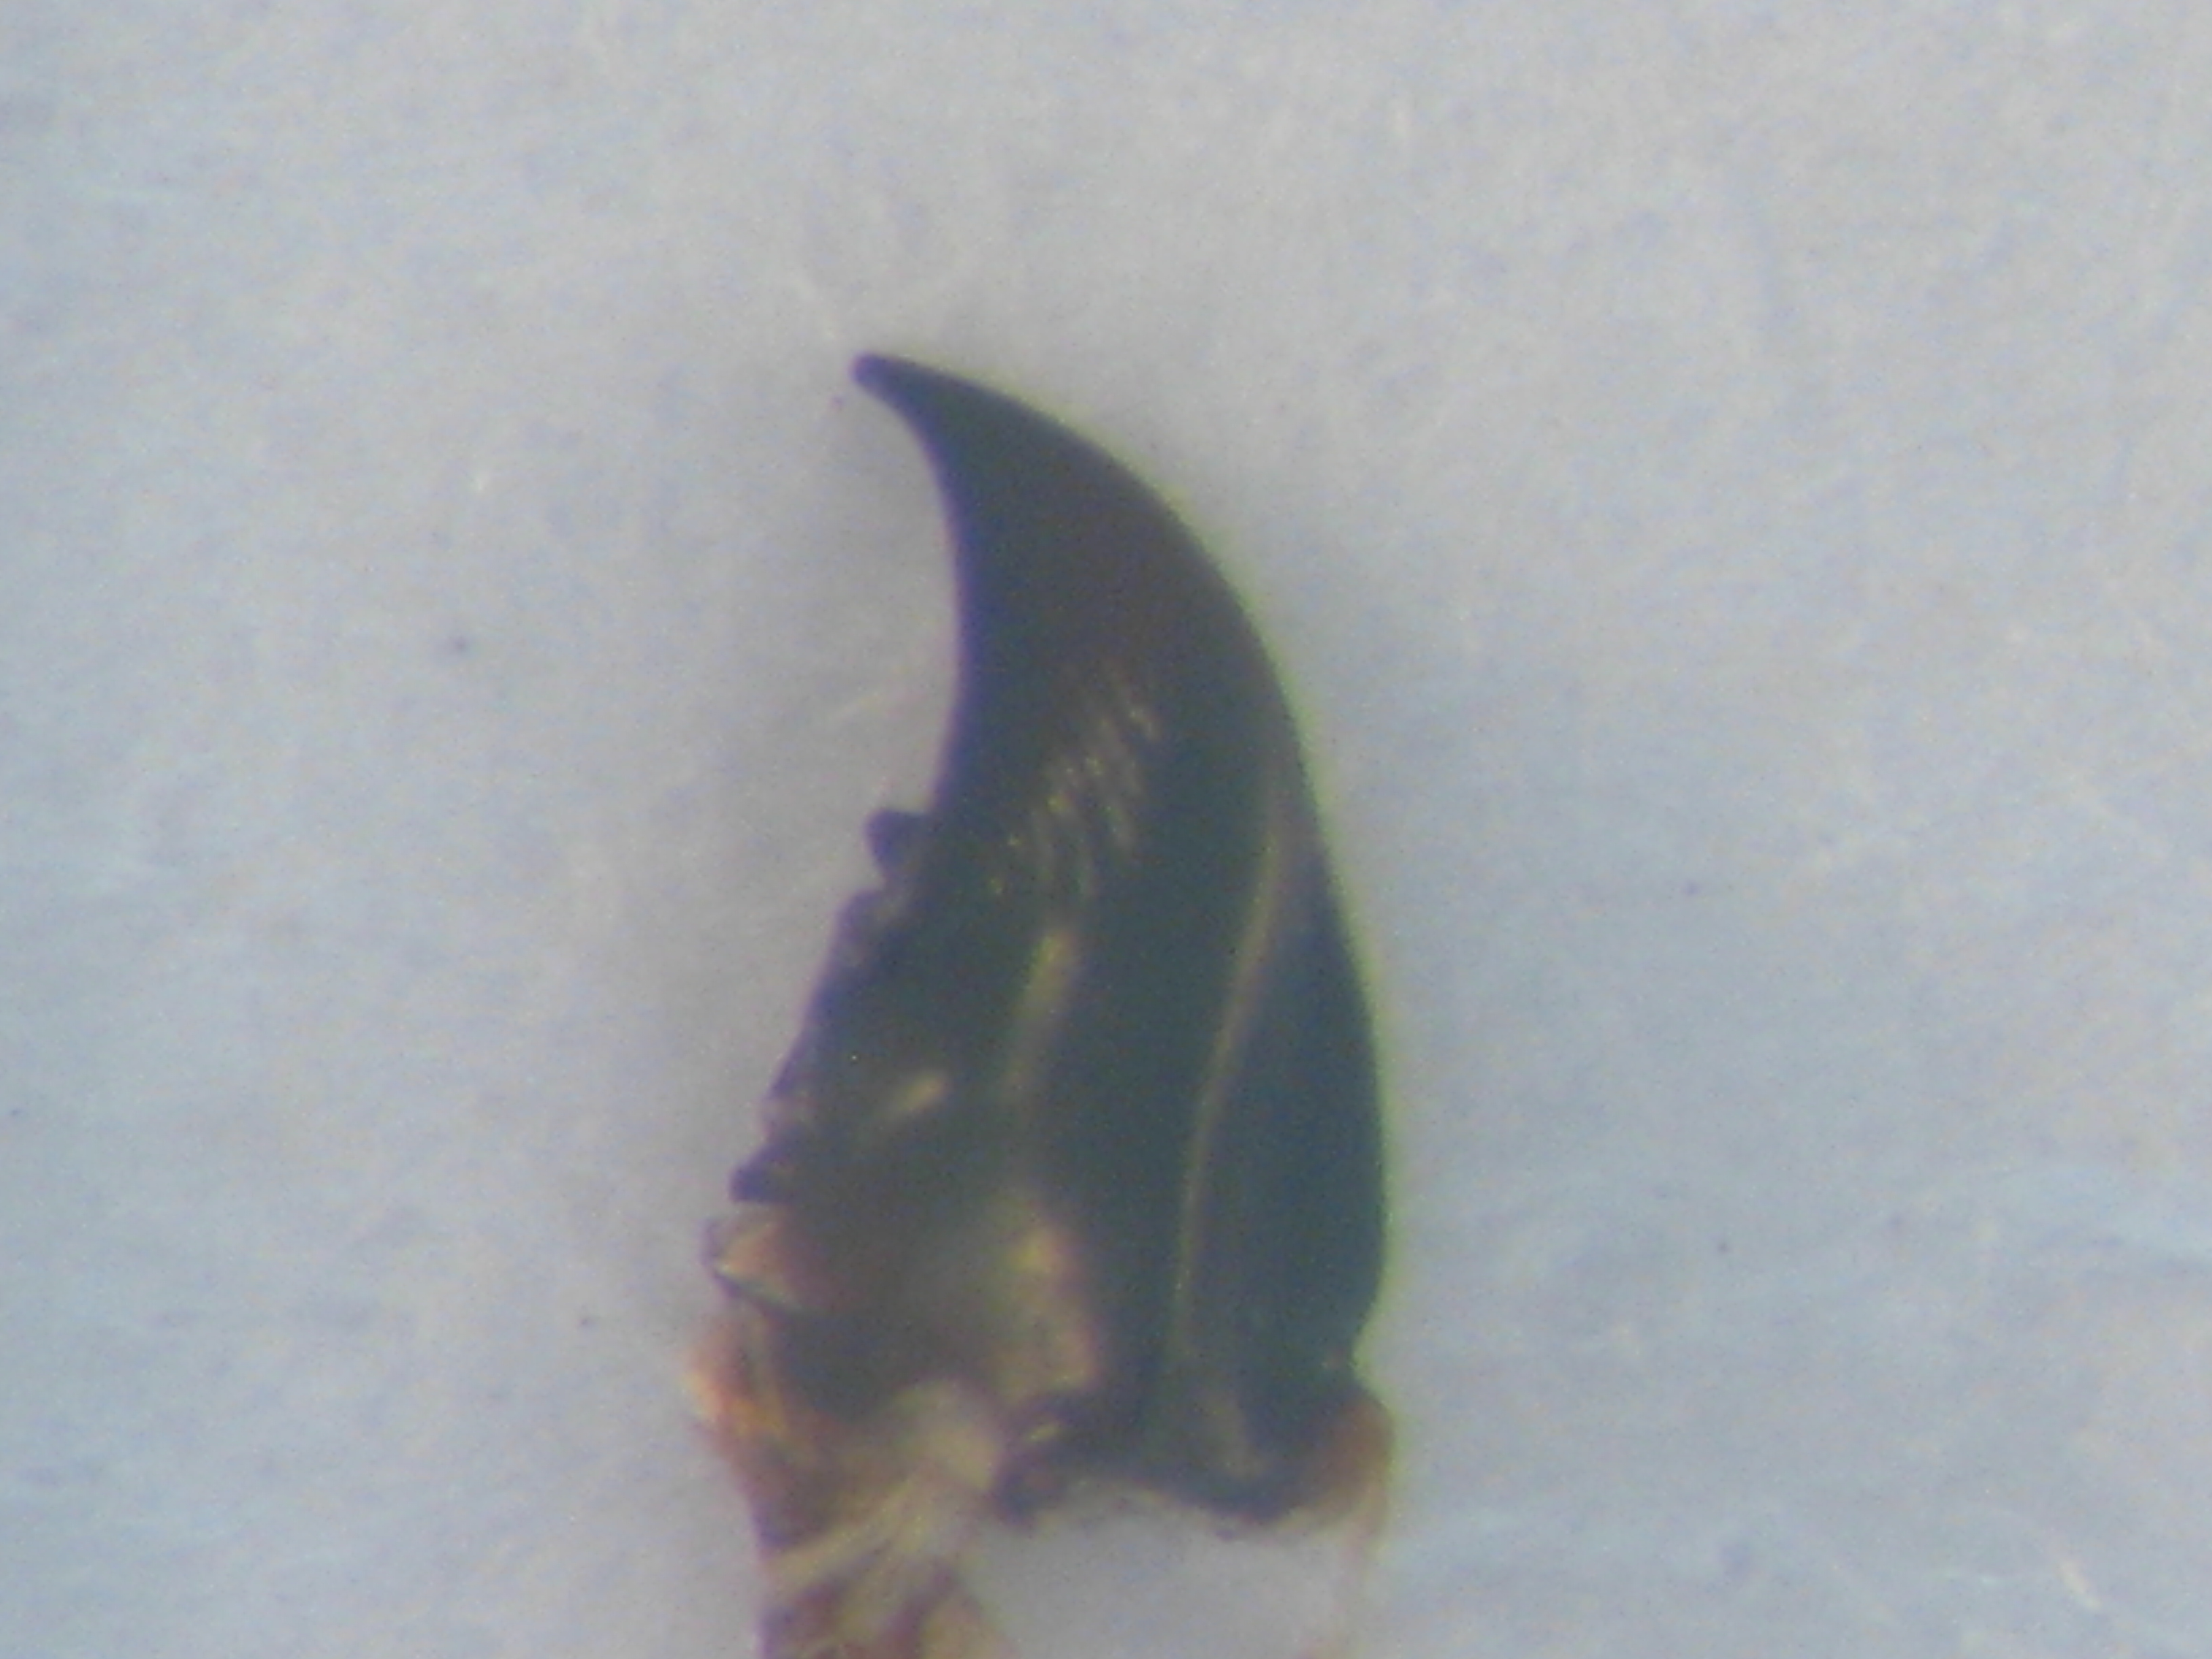
\includegraphics[width=0.45\textwidth]{./images/md32}}\\
\subfloat[The scene image with estimated landmarks by cross-correlation ]{\label{fig:462}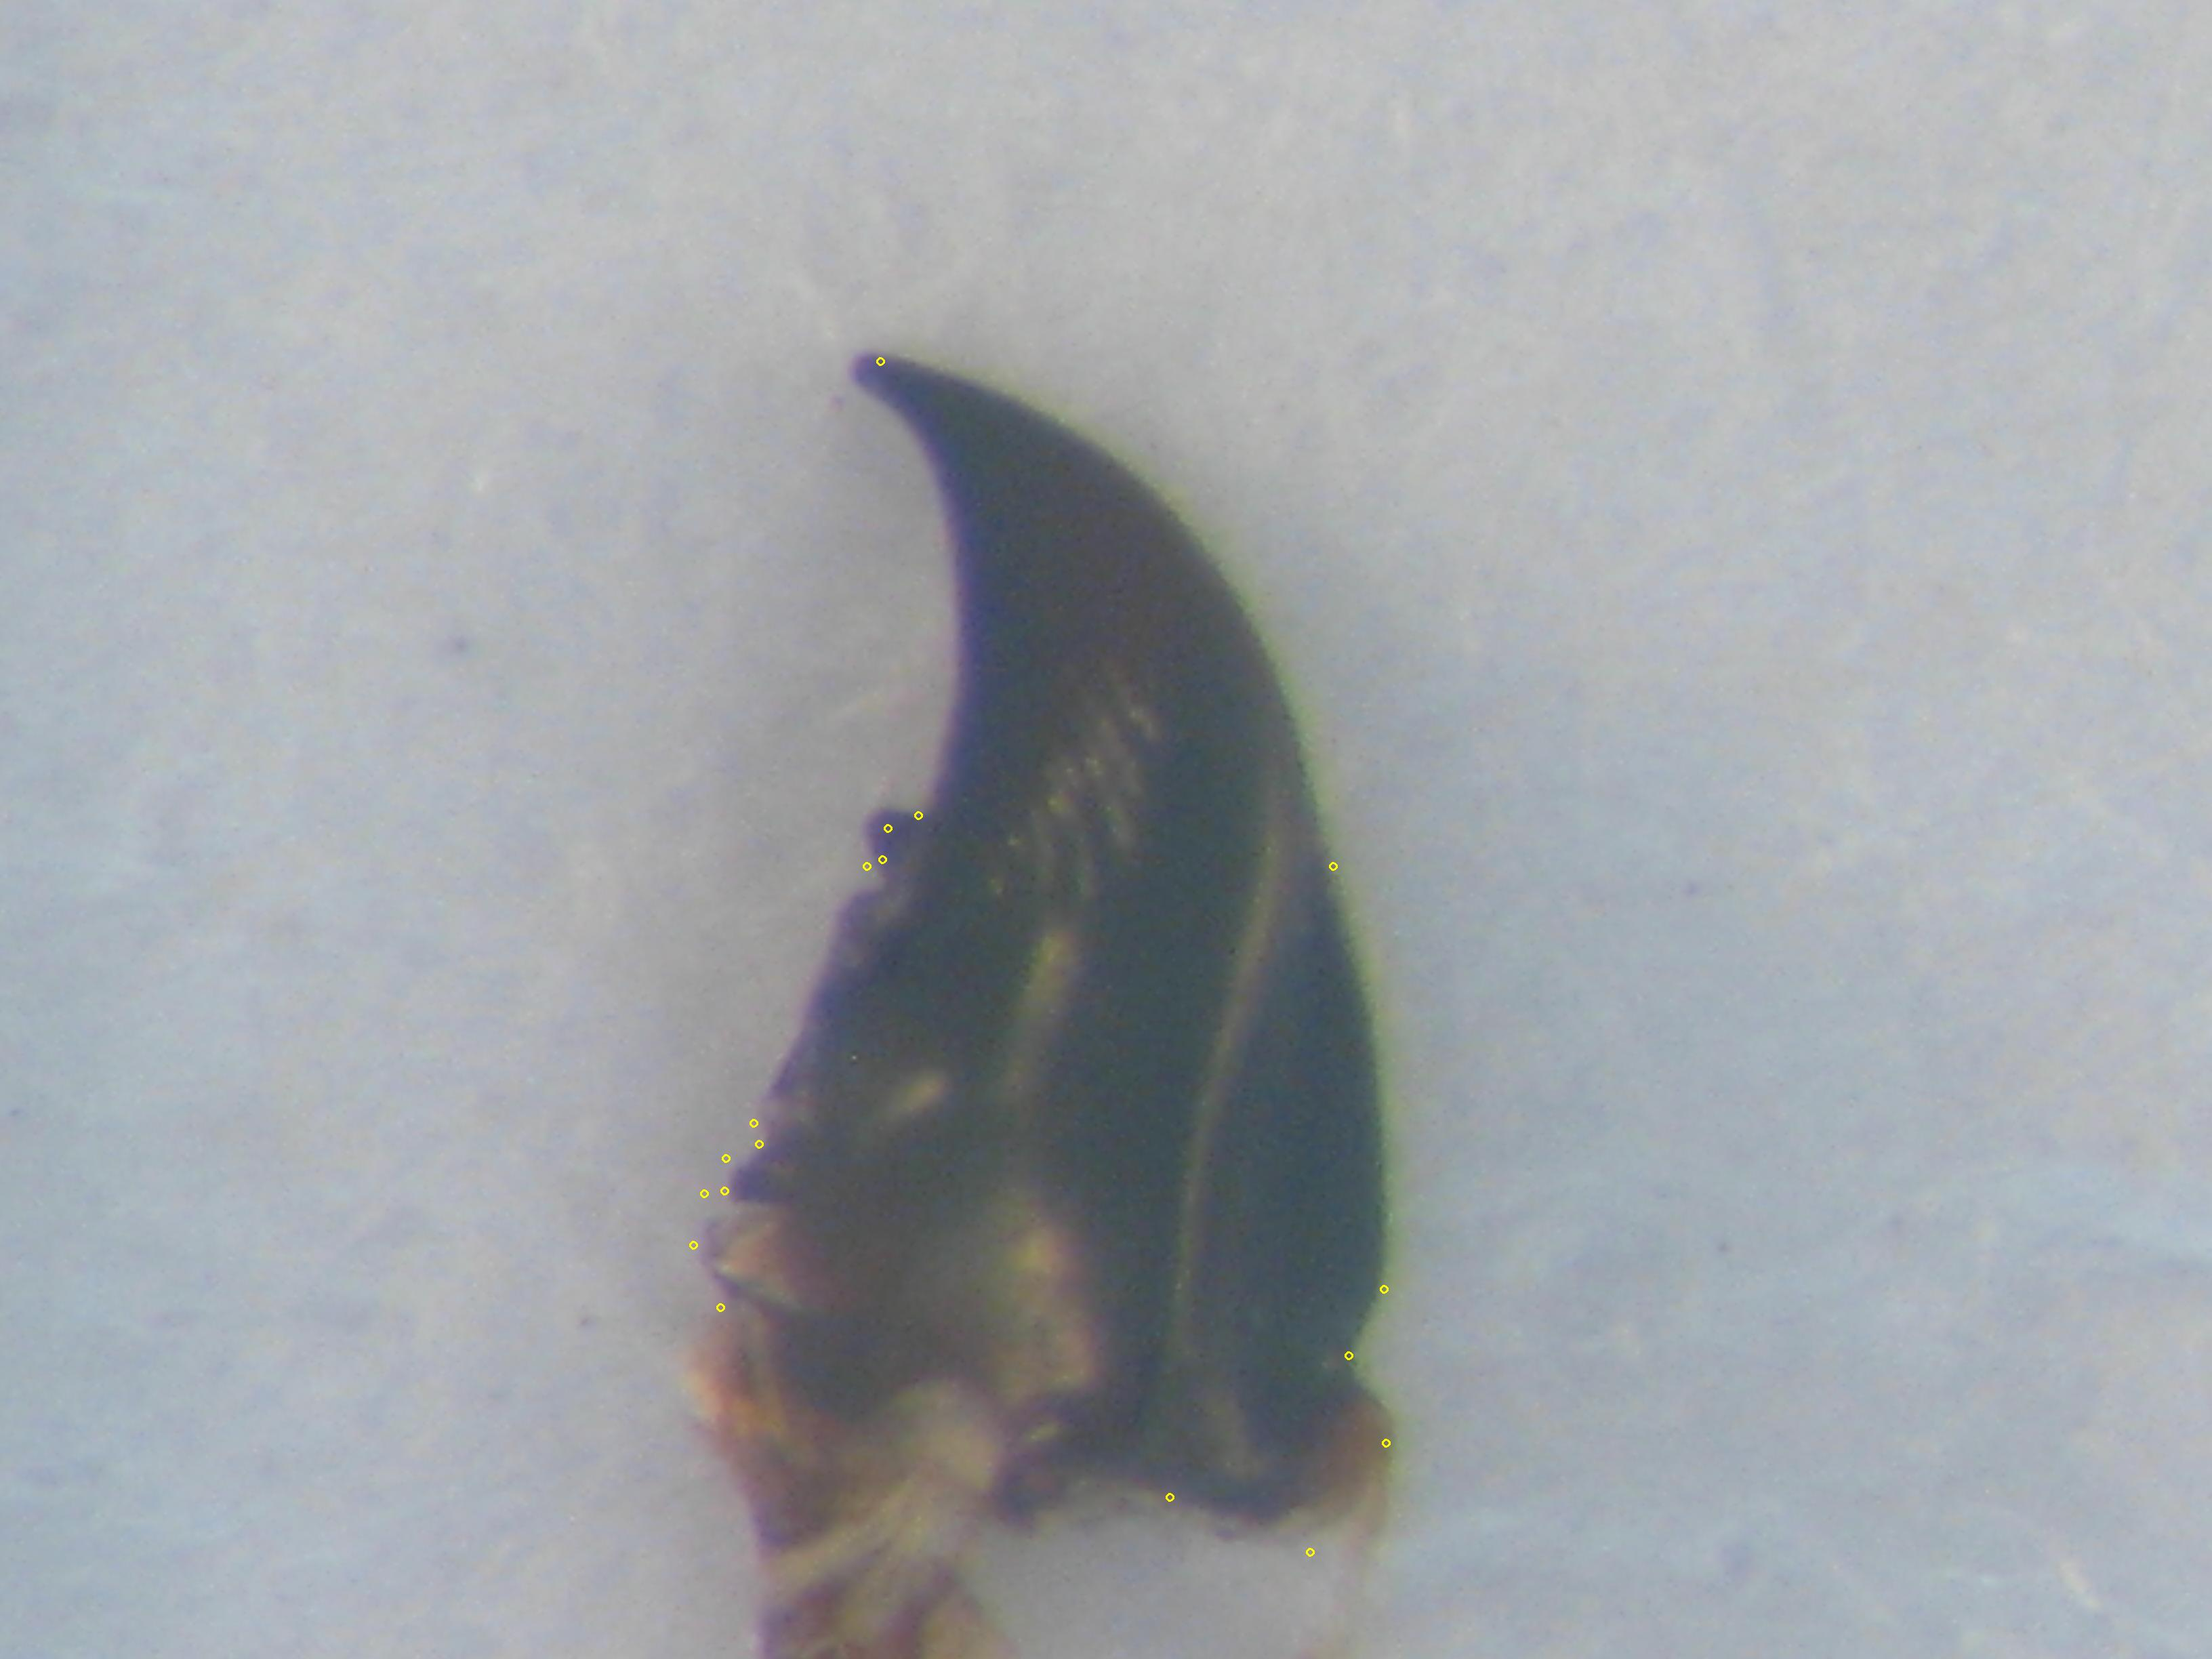
\includegraphics[width=0.45\textwidth]{./images/md32_cross}}~~
\subfloat[The scene image with estimated landmarks (by article) ]{\label{fig:463}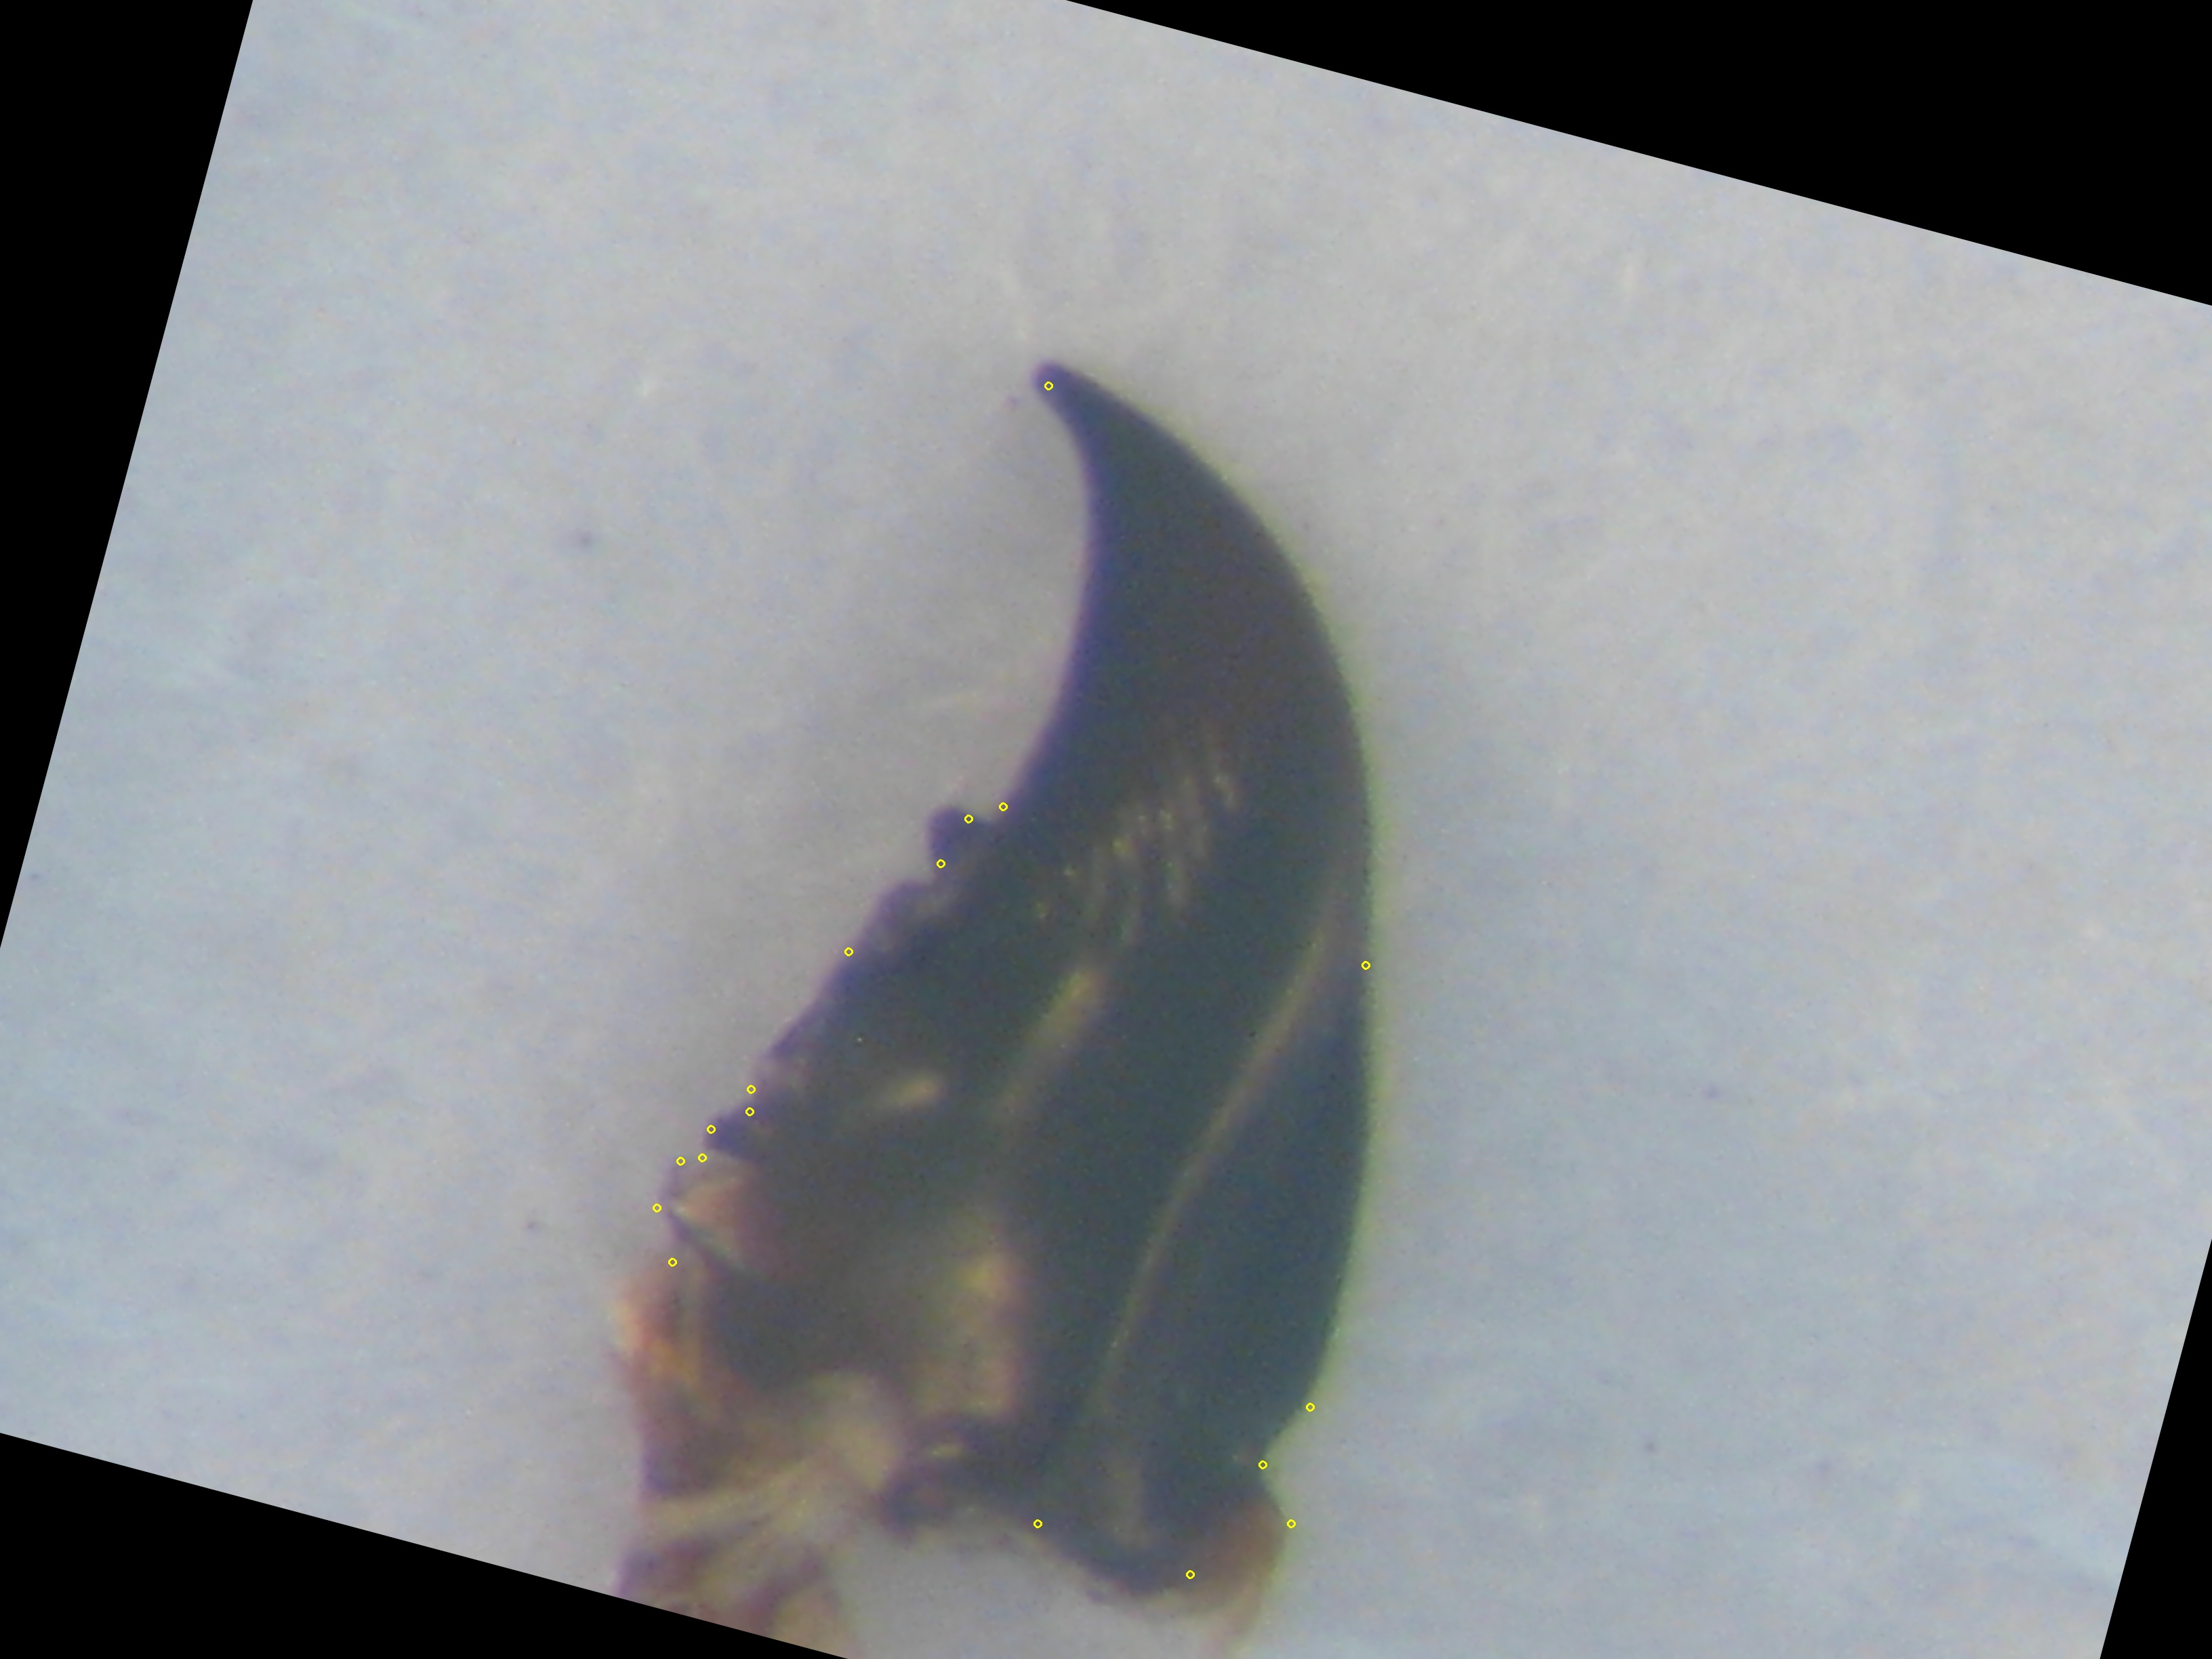
\includegraphics[width=0.45\textwidth]{./images/est32}}
\caption{Automatic identification of the landmarks}
\label{fig:46}
\end{figure}~\\
To have the basic evaluation about this method, we compare its result with the result from \textbf{``original"} of cross-correlation method. Obvious, the location of landmarks obtained from method (follows article) more closer than the landmarks obtained from cross-correlation (see in figure \ref{fig:46}).\\
Besides, the accuracy of the system can be determined by comparing the differences(in pixels) between the landmarks located by this method and the manual landmarks. This method has to pass several steps, the result of each step will effect on next steps. Thus, to evaluate the accuracy of this method, we can evaluate the result of each step.
\subsection{Limits and future works}
The method includes several steps to get the last result. At each step, we can use different ways to do. The methods proposed in this report just a part of them. Moreover, the program has use the parameters as the conditions, changing the values of parameters can effected to the accuracy of program.
Currently, the work finishes on two sets of data: \textit{right mandible} and \textit{left mandible}. In the future, we can evaluate and improve this method. Then applying this method on other dataset of biological images.
